% !TEX root =  ../../thesis.tex

\chapter{Simulation study}
\label{ch : simulation_study}

In this chapter we will share results from the simulation study we performed to check the efficacy of the model selection criteria described in Chapter \ref{ch : model_selection}. We implemented the Bayesian heterogeneity model using the R package R2jags \citep{su_r2jags:_2015} and analyzed the MCMC chains using the R package ggmcmc \citep{marin_ggmcmc:_2016}. For the calculation of marginal likelihood we required the density function of wishart distribution, which was available in two packages, namely MCMCpack and mixAK. There were inconsistencies in the results from the two implementations for extreme values of the wishart random variable. We eventually used mixAK \citep{komarek_mixak:_2015} as the MCMCpack package predicted density function value to be $\infty$ in some cases.

\section{Description of the data sets}
The data sets we simulated were motivated by the study on predicting Zebu cow's weights in sub saharan Africa \citep{lesosky_live_2012}. We assumed our response to be the weight of the Zebu cows. The predictors we considered were hypothetical, namely gender of a cattle (Male/Female), birth year of the cattle (1996/1997), age of the cattle at the first measurement and the time at which measurement was taken. The measurements of the cows were done at 10 different equally spaced time intervals. We further added subject specific random intercept and random slope effect to each response so that the repeated measurements for a given cow were correlated. Simulatenously we made sure that these cow specific random effects were mixture distributed. We will refer to the cows as subjects hereforth.

\subsection{Data sets for simulation study}
Our aim was to create data sets differing in number of mixture components for random effects, number of subjects, statistical power to detect the fixed effects, separation of mixture components, number of subjects per component. To analyze the efficacy of model selection criteria under these different scenarios we created the multiple data sets. To get a rough idea about the random effects in each of these data sets, we did graphical analysis. For this purpose we first regressed the response $\boldsymbol{y}$ on the 3 predictors age, gender and birth year of cattle using OLS. We then subjectwise regressed the residuals from OLS on the intercept and time of measurement to obtain a rough estimate of the random effect $\tilde{\boldsymbol{b}_i}$ of the $i^\text{th}$ subject. It is to be noted that this estimator overestimates the actual size of the random effects.

\subsubsection{Data set 1: No mixture distribution of random effects}
\label{subsubsec : ds_simple}
The first data set we created was without a mixture of random effects. i.e. $\boldsymbol{b}_i \sim N(0, G)$. In total we generated data of 80 subjects, each having 10 repetitions. Based on the approach mentioned above, a plot of the random effect values for this data set is shown in figure \ref{fig : ds_simple_randplot}.

\subsubsection{Data set 2: 3 well separated components for the mixture of random effects}
\label{subsubsec : ds_3wellsep}
The next data set we created had 3 well separated components forming the mixture distribution of random effects. In total we generated data of 180 subjects, each having 10 repetitions. A plot of the rough estimates of random effect values for this data set is shown in figure \ref{fig : ds_3wellsep_randplot}.

\begin{figure}[!htb]
\centering
	\begin{subfigure}[b]{0.4\textwidth}
		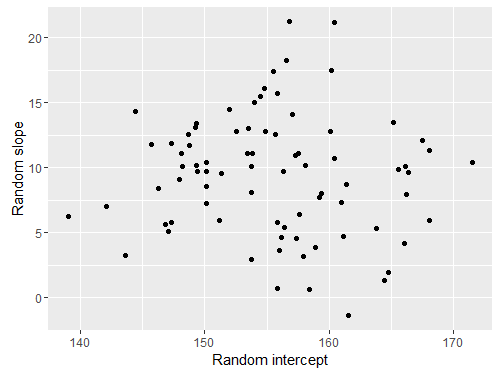
\includegraphics[width=\textwidth]{mainmatter/chapter_5_simulation_study/ds_simple_randplot.png}
       \caption{\label{fig : ds_simple_randplot}Data set 1}
	\end{subfigure}    
    \begin{subfigure}[b]{0.4\textwidth}
		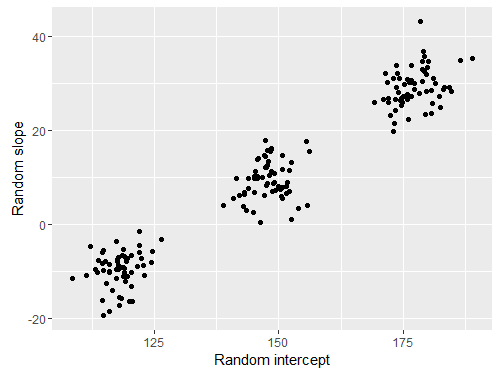
\includegraphics[width=\textwidth]{mainmatter/chapter_5_simulation_study/ds_3wellsep_randplot.png}
        \caption{\label{fig : ds_3wellsep_randplot}Data set 2}
	\end{subfigure}
\caption{\label{fig : ds_simple_n_3wellsep}Rough estimate $\tilde{\boldsymbol{b}_i}$ for random effects}
\end{figure}

\subsubsection{Data set 3: 3 well separated components but less subjects}
\label{subsubsec : ds_3wellsep_3ppg}
This data is similar to Data set 2 in all regards except for the number of subjects. We generated only 36 subjects in total in this data set. A plot of the rough estimates of random effect values for this data set is shown in figure \ref{fig : ds_3wellsep3ppg_randplot}.

\subsubsection{Data set 4: 3 fused components for the mixture of random effects}
\label{subsubsec : ds_3fused_10ppg}
In this data set we simulated the random effects from a mixture distribution which had 3 fused components. For e.g. if one sees the plot of the rough estimates of random effect values for this data set (figure \ref{fig : ds_3wellsep3ppg_randplot}) then it is likely that they select 1 or 2 components.

\begin{figure}[!htb]
\centering
	\begin{subfigure}[b]{0.4\textwidth}
		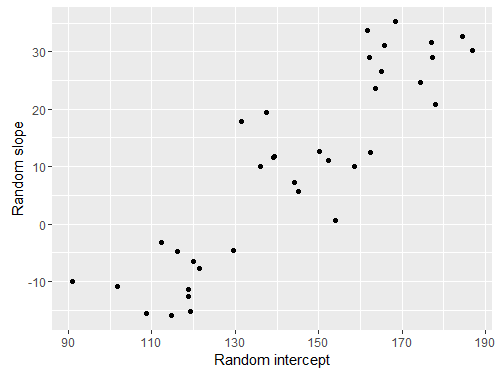
\includegraphics[width=\textwidth]{mainmatter/chapter_5_simulation_study/ds_3wellsep3ppg_randplot.png}
       \caption{\label{fig : ds_3wellsep3ppg_randplot}Data set 3}
	\end{subfigure}    
    \begin{subfigure}[b]{0.4\textwidth}
		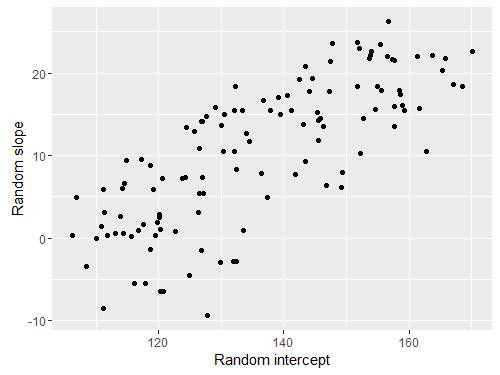
\includegraphics[width=\textwidth]{mainmatter/chapter_5_simulation_study/ds_3fused10ppg_randplot.png}
        \caption{\label{fig : ds_3fused10ppg_randplot}Data set 4}
	\end{subfigure}
\caption{\label{fig : ds_3comp_3ppgwelsep_10ppgfused}Rough estimate $\tilde{\boldsymbol{b}_i}$ for random effects}
\end{figure}

\subsubsection{Data set 5: 3 fused components but less subjects}
\label{subsubsec : ds_3fused_3ppg}
This data is similar to Data set 4 in all regards except for the number of subjects. We generated only 36 subjects in total in this data set. A plot of the rough estimates of random effect values for this data set is shown in figure \ref{fig : ds_3fused3ppg_randplot}.

\subsubsection{Data set 6: 5 well separated components}
\label{subsubsec : ds_5wellsep}
In this data set we simulated the random effects from a mixture distribution which had 5 well separated components. However this time we generated unequal number of subjects for every component. It is important to note that while we generated equal number of components per group earlier, depending upon how many components we model we might still deal with the problem of nearly empty components. The plot of the rough estimates of random effect values for this data set is shown in figure \ref{fig : ds_5wellsep_randplot}.

\begin{figure}[!htb]
\centering
	\begin{subfigure}[b]{0.4\textwidth}
		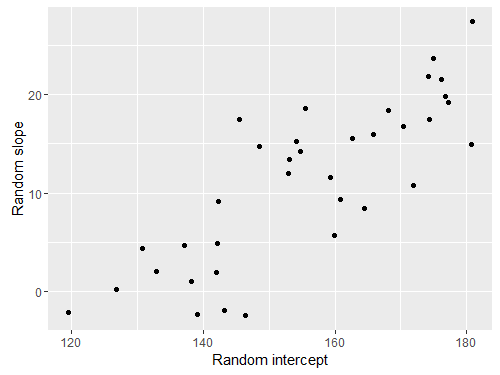
\includegraphics[width=\textwidth]{mainmatter/chapter_5_simulation_study/ds_3fused3ppg_randplot.png}
       \caption{\label{fig : ds_3fused3ppg_randplot}Data set 5}
	\end{subfigure}    
    \begin{subfigure}[b]{0.4\textwidth}
		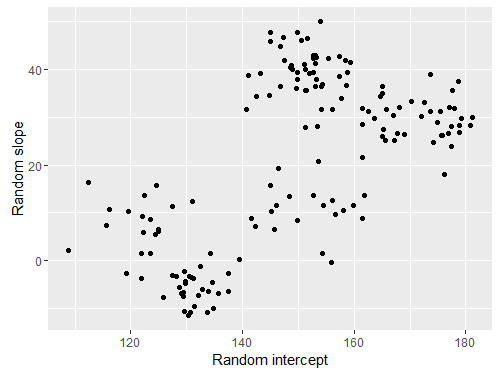
\includegraphics[width=\textwidth]{mainmatter/chapter_5_simulation_study/ds_5wellsep_randplot.png}
        \caption{\label{fig : ds_5wellsep_randplot}Data set 6}
	\end{subfigure}
\caption{\label{fig : ds_3fused3ppg_5wellsep}Rough estimate $\tilde{\boldsymbol{b}_i}$ for random effects}
\end{figure}

\subsubsection{Data set 7: 5 fused components}
\label{subsubsec : ds_5fused}
his data is similar to Data set 6 in all regards except that the number of subjects per component are lesser, and the components are not so well separated. The plot of the rough estimates of random effect values for this data set is shown in figure \ref{fig : ds_5fused_randplot}.

\begin{figure}[!htb]
\centering
	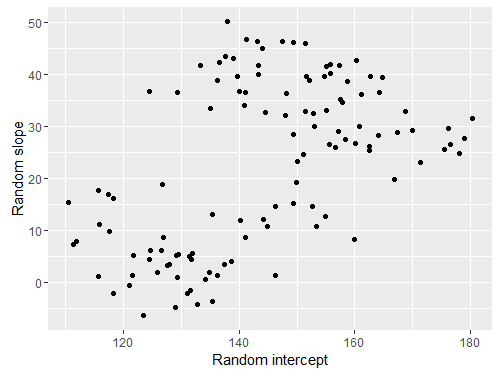
\includegraphics[scale=0.5]{mainmatter/chapter_5_simulation_study/ds_5fused_randplot.png}
	\caption{Rough estimate $\tilde{\boldsymbol{b}_i}$ for random effects of data set 7.}
	\label{fig : ds_5fused_randplot}    
\end{figure}


\subsection{Running MCMC simulations}
One of the primary issues we faced in running MCMC simulations were, label switching across chains, i.e. label 1 corresponding to component 1 in one chain and corresponding to some other component in another chain. This gave inconsistent and incorrect estimates for the various calculations we did. Although we dealt with it using the mechanism given in section \ref{subsec : label_switching_blmm}, it decreased the speed of simulations drastically. To make matters worse we had to use thinning of around 1 per 100 iterations to make sure the resulting chains were not autocorrelated. In light of these reasons and given the time constraints we had to be content with chains of 1300 iterations. MULTIPLE CHAINS,....CONSISTENT RESULTS.,...DIC results not based on a single chain.

\subsection{Deviance information criteria}
Table \ref{table : ds_simple_dic} shows the values of the various Deviance information criteria (section \ref{sec : dic}) applied to data set 1. We can see that $\text{DIC}_1$ gives misleading results whereas the rest of the DIC's remain more or less the same for overfitted models. The value of ${\text{p}_\text{D}}_1$ is negative (-602) when we fitted 3 components. \citet[pg. 161]{lunn_bugs_2012} noted that this can happen if the posterior is multimodal, which as we know can happen due to label switching when models are overfitted. For the same reason \citet{celeux_deviance_2006} suggest using $\text{DIC}_3$ instead of the other two observed data DIC measures.

\begin{table}[!htb]
\centering
\caption{DIC and $\text{p}_\text{D}$ for data set 1.}
\label{table : ds_simple_dic} 
\begin{tabular}{@{}rrrrrrr@{}}
\toprule
\# Comp Fitted & $\text{DIC}_1$ & $\text{DIC}_2$  & $\text{DIC}_3$  & $\text{DIC}_4$  & $\text{DIC}_5$  & $\text{DIC}_6$  \\ \midrule
1      & 4143 & 4144 & 4143 & 5160 & 4402 & 3483 \\
2      & 4146 & 4147 & 4145 & 5161 & 4403 & 3480 \\
3      & 3536 & 4148 & 4147 & 5163 & 4388 & 3465 \\
4      & 9    & 4151 & 4149 & 5166 & 4407 & 3485 \\ \bottomrule
\end{tabular}

\begin{tabular}{@{}rrrrrrr@{}}
\toprule
\# Comp Fitted & ${\text{p}_\text{D}}_1$ & ${\text{p}_\text{D}}_2$ & ${\text{p}_\text{D}}_3$ & ${\text{p}_\text{D}}_4$ & ${\text{p}_\text{D}}_5$ & ${\text{p}_\text{D}}_6$ \\ \midrule
1      & 9    & 9    & 9    & 903  & 145  & 125  \\
2      & 9    & 10   & 9    & 903  & 145  & 122  \\
3      & -602 & 9    & 8    & 901  & 126  & 107  \\
4      & 9    & 11   & 9    & 903  & 145  & 127  \\ \bottomrule
\end{tabular}
\end{table}

Table \ref{table : ds_3wellsep_dic} shows the values of various DIC applied to the data set 2. One of the patterns we inferred out of the results was that for $\text{DIC}_4$ the DIC values decrease continually by a very large margin till the right number of components are fitted, whereas after that the DIC either decreases by a relative smaller margin or remains more or less the same. The behavior of $\text{DIC}_5$ and $\text{DIC}_3$ is similar to $\text{DIC}_4$, however the large decrease in DIC that we observe for $\text{DIC}_4$ is not that large for them. However these patterns do not seem applicable to $\text{DIC}_1$ and $\text{DIC}_6$. For $\text{DIC}_1$ the pattern is that the values of ${\text{p}_\text{D}}_1$ become negative for 4 or more components, i.e. sign of overfitting as we discussed above.

\begin{table}[!htb]
\centering
\caption{DIC and $\text{p}_\text{D}$ for data set 2.}
\label{table : ds_3wellsep_dic} 
\begin{tabular}{@{}rrrrrrr@{}}
\toprule
\# Comp Fitted & $\text{DIC}_1$ & $\text{DIC}_2$  & $\text{DIC}_3$  & $\text{DIC}_4$  & $\text{DIC}_5$  & $\text{DIC}_6$  \\ \midrule
1 & 9966 & 9959 & 9965 & 12921 & 10531 & 7855 \\
2 & 9865 & 9849 & 9864 & 12498 & 10458 & 7860 \\
3 & 9664 & 9665 & 9663 & 11847 & 10244 & 7870 \\
4 & 9516 & 9654 & 9664 & 11834 & 10266 & 7888 \\
5 & 7370 & 9729 & 9666 & 11812 & 10277 & 7870 \\
6 & 9498 & 9661 & 9668 & 11833 & 10242 & 7857 \\ \bottomrule
\end{tabular}

\begin{tabular}{@{}rrrrrrr@{}}
\toprule
\# Comp Fitted & ${\text{p}_\text{D}}_1$ & ${\text{p}_\text{D}}_2$ & ${\text{p}_\text{D}}_3$ & ${\text{p}_\text{D}}_4$ & ${\text{p}_\text{D}}_5$ & ${\text{p}_\text{D}}_6$ \\ \midrule
1 & 9 & 2 & 8 & 2670 & 279 & 269 \\
2 & 15 & -1 & 14 & 2344 & 304 & 272 \\
3 & 21 & 21 & 20 & 1933 & 331 & 282 \\
4 & -125 & 13 & 23 & 1913 & 345 & 298 \\
5 & -2270 & 89 & 26 & 1889 & 355 & 280 \\
6 & -147 & 16 & 23 & 1912 & 321 & 269 \\ \bottomrule
\end{tabular}
\end{table}

Table \ref{table : ds_3wellsep_3ppg_dic} shows the values of the various DIC's applied to the data set 3. Firstly we can see that the pattern we inferred for $\text{DIC}_1$ above is not applicable here. Similar to the previous data set $\text{DIC}_6$ does not reveal any meaningful pattern. We can also see that the pattern of $\text{DIC}_5$ that we noted above is also not applicable here. However for $\text{DIC}_3$ and $\text{DIC}_4$ one can still see that the pattern of DIC decreasing by big margins till the right number of components are fitted, is still valid. Interestingly the margins have decreased as the sample size for this data set was only 36 subjects compared to the 180 subjects in data set 2.

\begin{table}[!htb]
\centering
\caption{DIC and $\text{p}_\text{D}$ for data set 3}
\label{table : ds_3wellsep_3ppg_dic}
\begin{tabular}{@{}rrrrrrr@{}}
\toprule
\# Comp Fitted & $\text{DIC}_1$ & $\text{DIC}_2$  & $\text{DIC}_3$  & $\text{DIC}_4$  & $\text{DIC}_5$  & $\text{DIC}_6$  \\ \midrule
1 & 2013 & 2012 & 2012 & 2611 & 2118 & 1570 \\
2 & 1989 & 1949 & 1987 & 2497 & 2013 & 1562 \\
3 & 1942 & 1942 & 1940 & 2339 & 2039 & 1571 \\
4 & 1943 & 1944 & 1942 & 2342 & 2034 & 1559 \\
5 & 1936 & 1940 & 1944 & 2344 & 2049 & 1580 \\
6 & 1695 & 1948 & 1945 & 2344 & 2053 & 1579 \\ \bottomrule
\end{tabular}

\begin{tabular}{@{}rrrrrrr@{}}
\toprule
\# Comp Fitted & ${\text{p}_\text{D}}_1$ & ${\text{p}_\text{D}}_2$ & ${\text{p}_\text{D}}_3$ & ${\text{p}_\text{D}}_4$ & ${\text{p}_\text{D}}_5$ & ${\text{p}_\text{D}}_6$ \\ \midrule
1 & 8 & 7 & 7 & 545 & 52 & 45 \\
2 & 14 & -26 & 12 & 465 & -20 & 35 \\
3 & 17 & 17 & 15 & 370 & 70 & 46 \\
4 & 16 & 17 & 15 & 370 & 62 & 34 \\
5 & 8 & 11 & 15 & 370 & 75 & 56 \\
6 & -235 & 17 & 15 & 368 & 77 & 53 \\ \bottomrule
\end{tabular}
\end{table}

Table \ref{table : ds_3fused_3ppg} shows the results of applying various DIC's to data set 4. So far we have observed that $\text{DIC}_3$ and $\text{DIC}_4$ can be used to detect the number of components. Since the components in this data set are fused, and the subjects count is moderately high the results following are interesting to analyze. Firstly, we can see that $\text{DIC}_4$ still follows the pattern we have discussed so far, but with $\text{DIC}_5$ it is a bit difficult to justify. i.e. even if the components are fused, $\text{DIC}_4$ may work well.
 
\begin{table}[!htb]
\centering
\caption{DIC and $\text{p}_\text{D}$ for data set 4}
\label{table : ds_3fused_10ppg_dic}
\begin{tabular}{@{}rrrrrrr@{}}
\toprule
\# Comp Fitted & $\text{DIC}_1$ & $\text{DIC}_2$  & $\text{DIC}_3$  & $\text{DIC}_4$  & $\text{DIC}_5$  & $\text{DIC}_6$  \\ \midrule
1 & 6568 & 6566 & 6566 & 8454 & 6899 & 5197 \\
2 & 6531 & 6523 & 6530 & 8263 & 6946 & 5253 \\
3 & 6497 & 6492 & 6497 & 8017 & 6898 & 5263 \\
4 & 6347 & 6480 & 6488 & 7955 & 6898 & 5253 \\
5 & 6321 & 6463 & 6485 & 7932 & 6743 & 5259 \\
6 & 6382 & 6329 & 6489 & 7948 & 6611 & 5259 \\ \bottomrule
\end{tabular}

\begin{tabular}{@{}rrrrrrr@{}}
\toprule
\# Comp Fitted & ${\text{p}_\text{D}}_1$ & ${\text{p}_\text{D}}_2$ & ${\text{p}_\text{D}}_3$ & ${\text{p}_\text{D}}_4$ & ${\text{p}_\text{D}}_5$ & ${\text{p}_\text{D}}_6$ \\ \midrule
1 & 9 & 8 & 8 & 1694 & 139 & 127 \\
2 & 14 & 7 & 13 & 1527 & 210 & 182 \\
3 & 20 & 14 & 19 & 1341 & 222 & 187 \\
4 & -115 & 17 & 26 & 1287 & 230 & 181 \\
5 & -138 & 4 & 26 & 1265 & 76 & 187 \\
6 & -81 & -134 & 26 & 1275 & -62 & 185 \\ \bottomrule
\end{tabular}
\end{table}

To see the patterns in further light, we decided to decrease the number of subjects to 36. Table \ref{table : ds_3fused_3ppg_dic} shows the corresponding results of DIC. At first glance one can see that the pattern we saw so far for $\text{DIC}_4$ doesn't exist anymore. However, the catch here is that these results are with a dirichlet prior $Dir(1, 1, ..., 1)$ for the weight distribution. When we fitted 2 or more components we found that the MCMC chains had not converged with this prior. Given the fused data set, even with fitting 2 components we risk unidentifiability due to empty components. Thus we changed the prior to $\text{Dir}(3, 3, ..., 3)$ and fitted for 2 and 3 components respectively. With 2 components we found $\text{DIC}_4$ = 2441 and $\text{p}_\text{D}$ = 461. Whereas $\text{DIC}_3$ was 1937 with $\text{p}_\text{D}$ = 14. Further fitting with 3 components we obtained $\text{DIC}_4$ = 2352 and $\text{DIC}_4$ = 2346 respective. In light of these results one can still justify the pattern we have observed for $\text{DIC}_4$ so far. An interesting result from this exercise was that using only $Dir(1, 1, ..., 1)$ can lead to severe underfitting. 

\begin{table}[!htb]
\centering
\caption{DIC and $\text{p}_\text{D}$ for data set 5.}
\label{table : ds_3fused_3ppg_dic}
\begin{tabular}{@{}rrrrrrr@{}}
\toprule
\# Comp Fitted & $\text{DIC}_1$ & $\text{DIC}_2$  & $\text{DIC}_3$  & $\text{DIC}_4$  & $\text{DIC}_5$  & $\text{DIC}_6$  \\ \midrule
1 & 1944 & 1943 & 1943 & 2500 & 1879 & 1364 \\
2 & 1936 & 1941 & 1945 & 2487 & 1919 & 1408 \\
3 & 1886 & -3353 & 1944 & 2453 & -$\infty$ & 1525 \\
4 & 1892 & 1904 & 1944 & 2439 & 1851 & 1389 \\
5 & 1902 & 1840 & 1942 & 2418 & 704 & 336 \\
6 & 1883 & 1919 & 1933 & 2371 & 2023 & 1538 \\ \bottomrule
\end{tabular}

\begin{tabular}{@{}rrrrrrr@{}}
\toprule
\# Comp Fitted & ${\text{p}_\text{D}}_1$ & ${\text{p}_\text{D}}_2$ & ${\text{p}_\text{D}}_3$ & ${\text{p}_\text{D}}_4$ & ${\text{p}_\text{D}}_5$ & ${\text{p}_\text{D}}_6$ \\ \midrule
1 & 9 & 7 & 7 & 510 & -110 & -119 \\
2 & 2 & 7 & 11 & 500 & -68 & -73 \\
3 & -42 & -5281 & 16 & 470 & -$\infty$ & 41 \\
4 & -34 & -22 & 18 & 459 & -130 & -93 \\
5 & -21 & -83 & 19 & 442 & -1272 & -1146 \\
6 & -31 & 5 & 19 & 407 & 59 & 55 \\ \bottomrule
\end{tabular}
\end{table}

Table 

\begin{table}[!htb]
\centering
\caption{DIC and $\text{p}_\text{D}$ for data set 6}
\label{table : ds_5wellsep_dic}
\begin{tabular}{@{}rrrrrrr@{}}
\toprule
\# Comp Fitted & $\text{DIC}_1$ & $\text{DIC}_2$  & $\text{DIC}_3$  & $\text{DIC}_4$  & $\text{DIC}_5$  & $\text{DIC}_6$  \\ \midrule
1 & 8982 & 8981 & 8980 & 11847 & 9251 & 6655 \\
2 & 8829 & 8827 & 8827 & 11327 & 9293 & 6838 \\
3 & 8745 & 8742 & 8744 & 11036 & 9251 & 6895 \\
4 & 8669 & 8672 & 8677 & 10737 & 9208 & 6925 \\
5 & 8649 & 8643 & 8648 & 10601 & 9165 & 6909 \\
6 & 8096 & 8697 & 8650 & 10594 & 9183 & 6923 \\
7 & 7770 & 8364 & 8651 & 10593 & 7613 & 6919 \\
8 & 8196 & 8640 & 8653 & 10597 & 9143 & 6927 \\ \bottomrule
\end{tabular}

\begin{tabular}{@{}rrrrrrr@{}}
\toprule
\# Comp Fitted & ${\text{p}_\text{D}}_1$ & ${\text{p}_\text{D}}_2$ & ${\text{p}_\text{D}}_3$ & ${\text{p}_\text{D}}_4$ & ${\text{p}_\text{D}}_5$ & ${\text{p}_\text{D}}_6$ \\ \midrule
1 & 9 & 9 & 7 & 2591 & -5 & -14 \\
2 & 14 & 13 & 12 & 2224 & 190 & 169 \\
3 & 20 & 16 & 19 & 2035 & 250 & 223 \\
4 & 19 & 23 & 27 & 1824 & 296 & 251 \\
5 & 31 & 26 & 30 & 1725 & 289 & 232 \\
6 & -520 & 81 & 33 & 1711 & 300 & 246 \\
7 & -848 & -254 & 34 & 1706 & -1274 & 244 \\
8 & -424 & 19 & 33 & 1711 & 257 & 248 \\ \bottomrule
\end{tabular}
\end{table}


\begin{table}[]
\centering
\caption{My caption}
\label{my-label}
\begin{tabular}{@{}rrrrrrr@{}}
\toprule
\# Comp Fitted & $\text{DIC}_1$ & $\text{DIC}_2$  & $\text{DIC}_3$  & $\text{DIC}_4$  & $\text{DIC}_5$  & $\text{DIC}_6$  \\ \midrule
1 & 6708 & 6707 & 6706 & 8819 & 6977 & 5071 \\
2 & 6606 & 6605 & 6604 & 8443 & 6946 & 5135 \\
3 & 6539 & 6538 & 6537 & 8178 & 6944 & 5204 \\
4 & 6506 & 6514 & 6521 & 8078 & 6915 & 5196 \\
5 & 6505 & 6500 & 6508 & 7984 & 6896 & 5202 \\
6 & 6465 & 6501 & 6510 & 7988 & 6895 & 5196 \\
7 & 6200 & 6500 & 6512 & 7989 & 6883 & 5190 \\
8 & 6448 & 6498 & 6516 & 7995 & 6901 & 5196 \\ \bottomrule
\end{tabular}

\begin{tabular}{@{}rrrrrrr@{}}
\toprule
\# Comp Fitted & ${\text{p}_\text{D}}_1$ & ${\text{p}_\text{D}}_2$ & ${\text{p}_\text{D}}_3$ & ${\text{p}_\text{D}}_4$ & ${\text{p}_\text{D}}_5$ & ${\text{p}_\text{D}}_6$ \\ \midrule
1 & 9 & 8 & 7 & 1903 & 61 & 53 \\
2 & 15 & 14 & 13 & 1636 & 139 & 120 \\
3 & 21 & 20 & 19 & 1456 & 221 & 185 \\
4 & 12 & 20 & 26 & 1381 & 218 & 176 \\
5 & 26 & 22 & 29 & 1308 & 220 & 182 \\
6 & -14 & 21 & 30 & 1307 & 214 & 176 \\
7 & -282 & 18 & 30 & 1305 & 198 & 168 \\
8 & -36 & 14 & 32 & 1307 & 213 & 175 \\ \bottomrule
\end{tabular}
\end{table}

\subsection{Marginal likelihood}
We implemented Chib's approximation mentioned in section \ref{sec : marginal_likelihood}. Table \ref{table : marginal_likelihood_results} shows the results of $\log{\hat{m}(\boldsymbol{y})}$ for the various data sets and the models fitted for them. One can see that there is no obvious pattern visible in these results to conclude the efficacy of Bayes factor in selection of a model. We had observed so far that given our data sets, the results of overfitting was label switching. However fitting 1 and 2 components did not have label switching and the chains had good convergence as well. However even if we take the cases where we had large number of observations and the components were well separated such as data set 6, we can see marginal likelihood prefers fitting 1 component over 2. Also the results of marginal likelihood for 3, 4 and 5 components for data set 6, are more or less the same. It is important to note that there is a higher margin of error in these results as the MCMC iterations were done multiple times for each data set and each component. However as we have already shown even for data sets where these chances were very less, marginal likelihood doesn't help choosing the right model.

\begin{table}[!htb]
\centering
\caption{$\log{\hat{m}(\boldsymbol{y})}$ for data set 1}
\label{table : marginal_likelihood_results} 
\begin{tabular}{rrrrrrrrr}
\toprule
Fitted & 1 Comp & 2 Comp & 3 Comp & 4 Comp & 5 Comp & 6 Comp & 7 Comp & 8 Comp \\\midrule
Data set 1 & -2120 & -2128 & -2139 & -2142 &  &  &  &  \\
Data set 2 & -5019 & -4989 & -4937 & -4925 & -4938 & $\infty$ &  &  \\
Data set 3 & -1038 & -1044 & -1042 & -645 & -1003 & $\infty$ &  &  \\
Data set 4 & -3317 & -3318 & -3322 & -3332 & -3348 & $\infty$ &  &  \\
Data set 5 & -1001 & -1016 & -1032 & -1041 & -1058 & $\infty$ &  &  \\
Data set 6 & -4545 & -4492 & -4477 & -4467 & -4473 & $\infty$ & -4498 & -3985 \\
Data set 7 & -3397 & -3379 & -3373 & -3380 & -2749 & $\infty$ & $\infty$ & -3416 \\ \bottomrule
\end{tabular}
\end{table}



